\documentclass[english,man]{apa6}

\usepackage{amssymb,amsmath}
\usepackage{ifxetex,ifluatex}
\usepackage{fixltx2e} % provides \textsubscript
\ifnum 0\ifxetex 1\fi\ifluatex 1\fi=0 % if pdftex
  \usepackage[T1]{fontenc}
  \usepackage[utf8]{inputenc}
\else % if luatex or xelatex
  \ifxetex
    \usepackage{mathspec}
    \usepackage{xltxtra,xunicode}
  \else
    \usepackage{fontspec}
  \fi
  \defaultfontfeatures{Mapping=tex-text,Scale=MatchLowercase}
  \newcommand{\euro}{€}
\fi
% use upquote if available, for straight quotes in verbatim environments
\IfFileExists{upquote.sty}{\usepackage{upquote}}{}
% use microtype if available
\IfFileExists{microtype.sty}{\usepackage{microtype}}{}

% Table formatting
\usepackage{longtable, booktabs}
\usepackage{lscape}
% \usepackage[counterclockwise]{rotating}   % Landscape page setup for large tables
\usepackage{multirow}		% Table styling
\usepackage{tabularx}		% Control Column width
\usepackage[flushleft]{threeparttable}	% Allows for three part tables with a specified notes section
\usepackage{threeparttablex}            % Lets threeparttable work with longtable

% Create new environments so endfloat can handle them
% \newenvironment{ltable}
%   {\begin{landscape}\begin{center}\begin{threeparttable}}
%   {\end{threeparttable}\end{center}\end{landscape}}

\newenvironment{lltable}
  {\begin{landscape}\begin{center}\begin{ThreePartTable}}
  {\end{ThreePartTable}\end{center}\end{landscape}}

  \usepackage{ifthen} % Only add declarations when endfloat package is loaded
  \ifthenelse{\equal{\string man}{\string man}}{%
   \DeclareDelayedFloatFlavor{ThreePartTable}{table} % Make endfloat play with longtable
   % \DeclareDelayedFloatFlavor{ltable}{table} % Make endfloat play with lscape
   \DeclareDelayedFloatFlavor{lltable}{table} % Make endfloat play with lscape & longtable
  }{}%



% The following enables adjusting longtable caption width to table width
% Solution found at http://golatex.de/longtable-mit-caption-so-breit-wie-die-tabelle-t15767.html
\makeatletter
\newcommand\LastLTentrywidth{1em}
\newlength\longtablewidth
\setlength{\longtablewidth}{1in}
\newcommand\getlongtablewidth{%
 \begingroup
  \ifcsname LT@\roman{LT@tables}\endcsname
  \global\longtablewidth=0pt
  \renewcommand\LT@entry[2]{\global\advance\longtablewidth by ##2\relax\gdef\LastLTentrywidth{##2}}%
  \@nameuse{LT@\roman{LT@tables}}%
  \fi
\endgroup}


  \usepackage{graphicx}
  \makeatletter
  \def\maxwidth{\ifdim\Gin@nat@width>\linewidth\linewidth\else\Gin@nat@width\fi}
  \def\maxheight{\ifdim\Gin@nat@height>\textheight\textheight\else\Gin@nat@height\fi}
  \makeatother
  % Scale images if necessary, so that they will not overflow the page
  % margins by default, and it is still possible to overwrite the defaults
  % using explicit options in \includegraphics[width, height, ...]{}
  \setkeys{Gin}{width=\maxwidth,height=\maxheight,keepaspectratio}
\ifxetex
  \usepackage[setpagesize=false, % page size defined by xetex
              unicode=false, % unicode breaks when used with xetex
              xetex]{hyperref}
\else
  \usepackage[unicode=true]{hyperref}
\fi
\hypersetup{breaklinks=true,
            pdfauthor={},
            pdftitle={An Extension of the QWERTY Effect: Not Just the Right Hand, Expertise and Typability Predict Valence Ratings of Words},
            colorlinks=true,
            citecolor=blue,
            urlcolor=blue,
            linkcolor=black,
            pdfborder={0 0 0}}
\urlstyle{same}  % don't use monospace font for urls

\setlength{\parindent}{0pt}
%\setlength{\parskip}{0pt plus 0pt minus 0pt}

\setlength{\emergencystretch}{3em}  % prevent overfull lines

\ifxetex
  \usepackage{polyglossia}
  \setmainlanguage{}
\else
  \usepackage[english]{babel}
\fi

% Manuscript styling
\captionsetup{font=singlespacing,justification=justified}
\usepackage{csquotes}
\usepackage{upgreek}

 % Line numbering
  \usepackage{lineno}
  \linenumbers


\usepackage{tikz} % Variable definition to generate author note

% fix for \tightlist problem in pandoc 1.14
\providecommand{\tightlist}{%
  \setlength{\itemsep}{0pt}\setlength{\parskip}{0pt}}

% Essential manuscript parts
  \title{An Extension of the QWERTY Effect: Not Just the Right Hand, Expertise
and Typability Predict Valence Ratings of Words}

  \shorttitle{QWERTY EFFECT EXTENSION}


  \author{Erin M. Buchanan\textsuperscript{1}~\& Kathrene D. Valentine\textsuperscript{2}}

  % \def\affdep{{"", ""}}%
  % \def\affcity{{"", ""}}%

  \affiliation{
    \vspace{0.5cm}
          \textsuperscript{1} Missouri State University\\
          \textsuperscript{2} University of Missouri  }

  \authornote{
    Erin M. Buchanan is an Associate Professor of Quantitative Psychology at
    Missouri State University. K. D. Valentine is a Ph.D.~candidate at the
    University of Missouri.
    
    Correspondence concerning this article should be addressed to Erin M.
    Buchanan, 901 S. National Ave, Springfield, MO 65897. E-mail:
    \href{mailto:erinbuchanan@missouristate.edu}{\nolinkurl{erinbuchanan@missouristate.edu}}
  }


  \abstract{Typing is a ubiquitous daily action for many individuals; yet, research
on how these actions have changed our perception of language is limited.
One such influence, deemed the QWERTY effect, is an increase in valence
ratings for words typed more with the right hand on a traditional
keyboard (Jasmin \& Casasanto, 2012). Although this finding is
intuitively appealing given both right handed dominance and the smaller
number of letters typed with the right hand, extension and replication
of the right side advantage is warranted. The present paper reexamined
the QWERTY effect within the embodied cognition framework (Barsalou,
1999) and found that the right side advantage is replicable to new
valence stimuli, along with findings supporting embodied cognition.
Further, when examining expertise, right side advantage interacted with
typing speed and typability (i.e., alternating hand key presses or
finger switches) portraying that both skill and our procedural actions
play a role in judgment of valence on words.}
  \keywords{expertise, embodied cognition, valence, QWERTY \\

    \indent Word count: 4419
  }





\usepackage{amsthm}
\newtheorem{theorem}{Theorem}
\newtheorem{lemma}{Lemma}
\theoremstyle{definition}
\newtheorem{definition}{Definition}
\newtheorem{corollary}{Corollary}
\newtheorem{proposition}{Proposition}
\theoremstyle{definition}
\newtheorem{example}{Example}
\theoremstyle{definition}
\newtheorem{exercise}{Exercise}
\theoremstyle{remark}
\newtheorem*{remark}{Remark}
\newtheorem*{solution}{Solution}
\begin{document}

\maketitle

\setcounter{secnumdepth}{0}



From its creation in 1868, to its appearance in our homes today, the
QWERTY keyboard has held the interest of psychologists. The process of
typing on a keyboard requires many procedures to function in tandem,
which creates a wealth of actions to research (Inhoff \& Gordon, 1997).
Rumelhart and Norman (1982)'s computer model of skilled typing is still
highly influential. They hypothesize that typing results from the
activation of three levels of cognition: the word level, the key press
level, and the response level. They believe that after word perception,
the word level is activated, causing the key press level to initiate a
schema of the letters involved in typing the word. This schema includes
the optimal position on the keyboard for that specific hand-finger
combination to move to at the appropriate time for individual
keystrokes. Concurrently, the response system sends feedback information
to initiate a key press motion when the finger is in the appropriate
space. Their theory proposes that schemata and motion activations occur
simultaneously, constantly pulling or pushing the hands and fingers in
the right direction.

While many studies have focused on errors in typing to investigate
response system feedback (Logan, 1999), Logan (2003) argued for parallel
activation of key presses. He examined the Simon effect to show more
than one letter is activated at the same time, and consequently, the
second key press motion is begun before the first key press is done. The
Simon effect occurs when congruent stimuli create faster responses than
incongruent stimuli, much like the Stroop task (Simon, 1990; Simon \&
Small, 1969). For example, if we are asked to type the letter \emph{f}
(a left handed letter), we type it faster if the \emph{f} is presented
on the left side of the screen. Similarly, Rieger (2004) reported
finger-congruency effects by altering a Stroop task: participants were
required to respond to centrally presented letters based on color-key
combinations. When the letter and color were congruent (i.e., a
right-handed letter was presented in the designated color for a right
response), the skilled typists' responses were faster than incongruent
combinations. Further, this effect was present when participants
responded to items with their hands crossed on the responding device,
suggesting the effect was expertise-based rather than
experiment-response based. These results imply that automatic actions
stimulate motor and imagery representations concurrently and may be
linked together in the brain (Hommel, Müsseler, Aschersleben, \& Prinz,
2001; Logan \& Zbrodoff, 1998; Rieger, 2004). This dual activation of
motor and imagined items is the basis for embodied cognition, a rapidly
expanding field in psychology (Barsalou, 1999; Salthouse, 1986).

\subsection{Embodied Cognition}\label{embodied-cognition}

While the mind was traditionally considered an abstract symbol processor
(Newell \& Simon, 1976), newer cognitive psychology theories focus on
the interaction between the brain's sensorimotor systems and mental
representations of events and objects (Barsalou, 1999; Zwaan, 1999). The
interplay between these systems has been found in both neurological
(Hauk, Johnsrude, \& Pulvermüller, 2004; Lyons et al., 2010; Tettamanti
et al., 2005) and behavioral research (Cartmill, Goldin-Meadow, \&
Beilock, 2012; Holt \& Beilock, 2006; Zwaan \& Taylor, 2006). Motor
representations of tasks are activated even when not specifically asked
to perform the task, and if the action is well-learned, the task is
perceived as pleasant (Beilock \& Holt, 2007; Ping, Dhillon, \& Beilock,
2009; Yang, Gallo, \& Beilock, 2009). For example, Beilock and Holt
(2007) asked novice and expert typists to pick which one of two letter
dyads they preferred, which were either different hand combinations
(\emph{CJ}) or same finger combinations (\emph{FV}). They found that
novices have no preference in selection, while expert typists more
reliably picked the combinations that were easier to type. To show that
this effect was due to covert motor representation activation, and thus,
expanding on findings from van den Bergh, Vrana, and Eelen (1990),
participants also made preference selections while repeating a key press
combination. When expert motor planning was distracted by remembering
the pattern presented, no preference for letter dyads was found,
indicating that the simultaneous activation of the motor representation
was necessary to influence their likability ratings. Similar embodied
findings have also been portrayed with emotionally charged sentences and
facial movements (Havas, Glenberg, \& Rinck, 2007), positive-negative
actions, such as head nodding or arm movements (Glenberg, Webster,
Mouilso, Havas, \& Lindeman, 2009; Ping et al., 2009), and
perceptuomotor fluency (Oppenheimer, 2008; Yang et al., 2009).

\subsection{Body Specificity
Hypothesis}\label{body-specificity-hypothesis}

Using an embodied framework, Casasanto (2009) has proposed that
handedness dictates preference because our representations of actions
are grounded in our physical interactions with the environment. In
several studies, he portrayed that handedness influenced preference for
spatial presentation (i.e., left handed individuals associate
\enquote{good} with left, while right handed individuals associate
\enquote{good} with right), which in turn influenced judgments of
happiness and intelligence and our decision making in hiring job
candidates and shopping. In all these studies, participants reliably
selected the hand-dominant side more often, which does not match
cultural or neurolinguistic representations of positive-is-right and
negative-is-left (Davidson, 1992). These findings imply that our
handedness is a motor expertise that causes ease of action on the
dominant side to positively influence our perceptions of items presented
on that side. Further, Casasanto (2011) compiled a review of body
specific actions and their representation in the brain using fMRIs.
Handedness interacted with imagining actions, reading action, and
perceiving the meanings of action verbs, such that fMRI patterns were
mirrored for left and right handed participants matching their dominant
side.

\subsection{The QWERTY Effect}\label{the-qwerty-effect}

These effects lead Jasmin and Casasanto (2012) to propose the idea that
typing, an action that often replaces speaking, has the ability to
create semantic changes in how we perceive words. The asymmetrical
arrangement of letters on the QWERTY keyboard increases fluency of
typing letters on the right side because there are fewer keys, and thus,
less competition for fingers. That arrangement should then cause us to
perceive the letters on the right side as more positive and letters on
the left side as more negative. Consequently, words that are composed of
more letters from the right side (the right side advantage; RSA) should
be rated as more positive than those with more letters on the left. They
found this preference for RSA over three languages (English, Spanish,
and Dutch), and the effect was even stronger on words created after the
invention of the QWERTY keyboard (i.e., \emph{lol}), as well as evident
in pseudowords such as \emph{plook.} However, in contrast to the body
specificity hypothesis, left and right handed participants showed the
same trend in effects for positive-is-right words.

\section{Current Study}\label{current-study}

The current study examined the right side advantage's interaction with
traditional embodied cognition definitions (expertise, fluency). We
analyzed the different implications of the body specificity hypothesis
and a more general embodied hypothesis by testing the following:

\begin{enumerate}
\def\labelenumi{\arabic{enumi})}
\tightlist
\item
  Expertise was measured through participant typing speed, and fluency
  or typability was measured through finger and hand switches that would
  occur if the word was typed on a QWERTY keyboard (akin to Beilock and
  Holt (2007)'s different hand preferences). Given that typing involves
  the procedural action system, we would expect to find that increased
  hand and finger switches are positively related to ratings of valence
  because words that are typed on alternating fingers and hands are
  easier to type. It was unclear if expertise would directly influence
  overall ratings, as we expected an interaction of the variables
  (described below). The RSA may still be present when accounting for
  these variables, as humans are primarily a right side dominant
  species.
\item
  The interaction between RSA, hand and fingers switches, and expertise
  was examined to determine if these hypotheses can be combined. This
  analysis allowed us to explore the nuance of skill and typability on
  valence ratings and to determine the effects of the RSA at different
  levels these variables.
\end{enumerate}

\section{Method}\label{method}

\subsection{Participants}\label{participants}

Participants (\emph{N} = 606) were recruited from the undergraduate
human subject pool at a large Midwest university and received course
credit for their time. 72433 rows of data were present for these
participants, where 564 participants had complete data (i.e., 120 rows,
see below), 39 were missing one data point, and 3 were missing many data
points. All possible data points were considered and missing data points
were usually computer error (i.e., freezing during the experiment) or
participant error (i.e., missed key press).

Rating data were screened for multivariate outliers, and two
participant's ratings were found to have extreme Mahalanobis distance
scores (Tabachnick \& Fidell, 2012) but were kept in the data set. 11.2
percent of the sample was left-handed, 0.2 percent marked ambidextrous,
and 0.3 percent was missing handedness information. The average typing
speed was 47.89 words per minute (\emph{SD} = 13.31), and the average
percent accuracy rate for the typing test was 92.69 (\emph{SD} = 8.36).

\subsection{Materials}\label{materials}

The English ANEW (Bradley \& Lang, 1999) norms were used to create the
stimuli for this study, in an effort to replicate Jasmin and Casasanto
(2012) experiments, and 2743 words were selected for this experiment.
Pseudowords were selected from Appendix E of the supplementary materials
presented from the QWERTY publication. These words were coded as
described below for RSA, finger and hand switches, word length, and
letter frequency. Average word length was 4.75 (\emph{SD} = 1.47; range
= 3 - 13). All materials, data, and the \emph{R}markdown document that
created this manuscript are available at our Open Science Foundation
(OSF) page: \url{https://osf.io/zs2qj/}.

\subsection{Coding}\label{coding}

Each of the words used in this study were coded for control and
experimental variables. Control variables included word length and
average letter frequency. Average letter frequency was created by
averaging the English letter frequency (Lewand, 2000) for each letter in
a word. Words with high average letter frequencies contain more commonly
used letters (\emph{e, t, a, o}); while words with lower frequencies use
more of the less common letters (\emph{z, q, x, j}). Experimental
variables included RSA, number of hand switches, and number of finger
switches. Typing manuals were consulted, and letters were coded as left
(\emph{q, w, e, r, t, a, s, d, f, g, z, x, c, v, b}) or right-handed
letters (\emph{y, u, i, o, p, h, j, k, l, n, m}). Left handed letters
were coded with -1 and right handed letters with +1, which created
summed scores indicating the overall right side advantage for a word.
Words were coded for the number of hand switches within a word using the
left-right coding system described above. Finally, the number of finger
switches were coded using traditional typing manuals for each finger.
Finger switches was highly correlated with word length, \emph{r} = .89,
and therefore, word length was excluded as a control variable due to
focus on typing skill in our hypotheses.

\subsection{Procedure}\label{procedure}

Upon consent to participate in the experiment, participants were given a
typing test by using a free typing test website (TypingMaster, 2013).
Each participant typed Aesop's Fables for one minute before the website
would reveal their typing speed and accuracy rate, which was recorded by
the experimenter. After this test, participants indicated their dominant
writing hand. Participants were then given 120 of the possible stimuli
to rate for pleasantness (60 real words, 60 pseudowords). This smaller
number of stimuli was used to control fatigue/boredom on participants.
These stimuli were counterbalanced across participants, and the order of
the stimuli was randomized. Participants were told to rate each word for
how pleasant it seemed using a 9 point Likert type scale (1 - \emph{very
unpleasant}, 4 - \emph{neutral}, 9 - \emph{very pleasant}). The same
self-assessment manikin from Jasmin and Casasanto (2012) was shown to
participants at the top of the computer screen to indicate the points on
the Likert scale. The words appeared in the middle of the screen in 18
point Arial font. Participants then typed the number of their rating on
the computer keyboard. Once they rated all stimuli, participants were
debriefed and allowed to leave.

\section{Results}\label{results}

\subsection{Data Analytic Plan}\label{data-analytic-plan}

Because each participant constituted multiple data points within the
dataset, a multilevel model was used to control for correlated error
(Gelman, 2006). Pinheiro, Bates, Debroy, Sarkar, and Team (2017)'s
\emph{nlme} package in \emph{R} was used to calculate these analyses. A
maximum likelihood multilevel model was used to examine hypotheses of
interactions between typing speed, hand/finger switching, and RSA while
adjusting for letter frequency when predicting item pleasantness
ratings. Pseudowords and real words were examined separately in two
multilevel model analyses. Participants were included as a random
intercept factor, as comparison to a non-random intercept was
significant (see Table \ref{tab:model-table1}). Typing speed,
finger/hand switches, and RSA were mean centered before analyses to
control for multicollinearity.

\subsection{Main Effects}\label{main-effects}

After setting participants as a random intercept factor, letter
frequency was used as an adjustor variable. As seen in Table
\ref{tab:model-table1}, this variable was not a significant predictor
for pseudowords, \emph{b} = -0.006, but was a significant predictor for
real words, \emph{b} = 0.056. All predictor statistics are provided in
an Excel sheet on the OSF page for each step of the model. Next, the
main effects of typing speed, hand switches, finger switches, and RSA
were added to the models for pseudowords and real words. In both models,
the addition of these variables overall was significant, \emph{p}
\textless{} .001. For pseudowords, typing speed was not a significant
predictor of valence ratings, \emph{b} = 0.003, \emph{t}(601) = 0.97,
\emph{p} = .332. Similarly, typing speed was not a significant predictor
for valence ratings on real words, \emph{b} = 0.000, \emph{t}(604) =
0.04, \emph{p} = .971. In contrast, the measures of typability in hand
and finger switching were significant for both pseudowords and real
words. For pseudowords, increased hand switching, \emph{b} = -0.026,
\emph{t}(35535) = -2.84, \emph{p} = .004, and increased finger
switching, \emph{b} = -0.074, \emph{t}(35535) = -5.85, \emph{p}
\textless{} .001, decreased the overall valence ratings. However
increased hand switching, \emph{b} = 0.061, \emph{t}(35681) = 4.71,
\emph{p} \textless{} .001, increased valence ratings for real words,
while increased finger switching, \emph{b} = -0.091, \emph{t}(35681) =
-7.82, \emph{p} \textless{} .001, decreased the overall valence ratings.
Even adjusting for these typing style variables, the RSA effect
replicated for both pseudowords, \emph{b} = 0.050, \emph{t}(35535) =
11.50, \emph{p} \textless{} .001, and real words, \emph{b} = 0.051,
\emph{t}(35681) = 8.35, \emph{p} \textless{} .001. In the next section,
we explored the interactions of typability and RSA, to present a more
nuanced view of typing's effect on valence ratings.

\subsection{Interactions}\label{interactions}

\begin{table}[tbp]
\begin{center}
\begin{threeparttable}
\caption{\label{tab:model-table1}Area under curve model statistics}
\begin{tabular}{lccccccc}
\toprule
Word Type & Model & $df$ & AIC & BIC & $\chi^2$ & $\Delta\chi^2$ & $p$\\
\midrule
Pseudo & Intercept Only & 2 & 144345.73 & 144362.72 & -72170.87 & NA & NA\\
Pseudo & Random Intercept & 3 & 134813.09 & 134838.57 & -67403.54 & 9534.65 & < .001\\
Pseudo & Adjustor Variable & 4 & 134814.22 & 134848.20 & -67403.11 & 0.87 & .351\\
Pseudo & Main Effects & 8 & 134577.92 & 134645.89 & -67280.96 & 244.29 & < .001\\
Pseudo & Interactions & 19 & 134577.46 & 134738.87 & -67269.73 & 22.47 & .021\\
Real & Intercept Only & 2 & 168169.14 & 168186.14 & -84082.57 & NA & NA\\
Real & Random Intercept & 3 & 166459.55 & 166485.05 & -83226.78 & 1711.59 & < .001\\
Real & Adjustor Variable & 4 & 166424.46 & 166458.46 & -83208.23 & 37.09 & < .001\\
Real & Main Effects & 8 & 166281.81 & 166349.81 & -83132.91 & 150.65 & < .001\\
Real & Interactions & 19 & 166253.65 & 166415.14 & -83107.82 & 50.16 & < .001\\
\bottomrule
\addlinespace
\end{tabular}
\begin{tablenotes}[para]
\textit{Note.} AIC: Aikaike Information Criterion, BIC: Bayesian Information Criterion
\end{tablenotes}
\end{threeparttable}
\end{center}
\end{table}

Next, the four-way interaction of typing speed, finger switching, hand
switching, and RSA was entered into the equation, including all the
smaller two- and three-way interactions. We focused on the most complex
interaction found, breaking down interaction terms into simple slopes of
low (-1SD), average, and high (+1SD) to explore each effect. For
example, if the four-way interaction was significant, one variable would
be broken into simple slopes, and the next most complex interactions
would be examined. This procedure was iterated until the interactions
were no longer significant or only main effects were examined. When
multiple interactions were present, we choose a common variable to help
break down the interactions with the least number of steps. Table
\ref{tab:model-table1} portrays that the addition of the interaction
components was significant for both pseudoword, \emph{p} = .003, and
real word, \emph{p} \textless{} .001, models.

\subsubsection{Pseudoword Simple Slopes}\label{pseudoword-simple-slopes}

For pseudowords, finger switches by RSA, \emph{b} = 0.014,
\emph{t}(35524) = 2.66, \emph{p} \textless{} .001, and typing speed by
RSA, \emph{b} = -0.001, \emph{t}(35524) = -2.00, \emph{p} = .045 were
the only significant interactions. Low and high simple slopes for RSA
were created to examine the effects of typing speed and finger switches
at these levels, and these interactions are displayed in Figure
\ref{fig:graphs}. For low RSA (words with more left handed letters),
speed positively predicted valence, \emph{b} = 0.007, \emph{t}(541) =
2.08, \emph{p} = .038, and finger switching negatively predicted
valence, \emph{b} = -0.094, \emph{t}(31984) = -5.29, \emph{p}
\textless{} .001. For average RSA, speed no longer predicted valence,
\emph{b} = 0.003, \emph{t}(601) = 1.07, \emph{p} = .285, while finger
switches still negatively predicted valence, albeit to a lesser extent
than at low RSA, \emph{b} = -0.062, \emph{t}(35524) = -4.76, \emph{p}
\textless{} .001. Last, at high RSA (more right handed words), speed did
not predict valence, \emph{b} = 0.002, \emph{t}(541) = 0.62, \emph{p} =
.536, and neither did finger switches, \emph{b} = -0.002,
\emph{t}(31984) = -0.09, \emph{p} = .926. In sum, this interaction
indicated that expertise may be seen as positively influencing ratings
for more left handed words, but was not a predictor of words that were
typed more with the right hand. When words were more left handed, there
was a negative influence of finger switching, but as we transition to
more right handed words the number of switches did not influence valence
ratings. These results seemed to indicate that expertise and typability
were influential factors for left handed words, but the RSA washed out
these effects when rating right handed pseudowords.

\subsubsection{Real Word Simple Slopes}\label{real-word-simple-slopes}

For real words, the three-way interactions of finger switch by hand
switch by RSA, \emph{b} = -0.009, \emph{t}(35670) = -5.00, \emph{p}
\textless{} .001, and speed by finger switch by hand switch, \emph{b} =
-0.001, \emph{t}(35670) = -2.62, \emph{p} = .009, were the largest
significant interaction predictors. Low and high simple slopes for
finger switches were created to explore the three-way interaction. For
lower finger switches, the hand switching by RSA interaction was
significant, \emph{b} = 0.024, \emph{t}(32130) = 2.81, \emph{p} = .005;
however, the hand switches by speed interaction was not significant,
\emph{b} = 0.001, \emph{t}(32130) = 0.43, \emph{p} = .664. At average
finger switching, the hand switches by RSA interaction was not
significant, \emph{b} = -0.002, \emph{t}(35670) = -0.38, \emph{p} =
.705, and neither was the hand switches by speed interaction, \emph{b} =
-0.001, \emph{t}(35670) = -1.21, \emph{p} = .228. At a higher number of
finger switches the hand switches by RSA interaction was significant,
\emph{b} = -0.016, \emph{t}(32130) = -2.91, \emph{p} = .004, along with
the hand switches by speed interaction, \emph{b} = -0.001,
\emph{t}(32130) = -2.64, \emph{p} = .008.

For significant two-way effects of hand switch by RSA and hand switch by
speed, we then calculated the low and high simple slopes for hand
switches, see Figure \ref{fig:graphs2}. Therefore, we explored the low
and high finger switch effects that were significant with low and high
hand switches for RSA and speed main effects. At low finger switches and
low hand switches, RSA was a significant predictor of valence, \emph{b}
= 0.026, \emph{t}(32130) = 2.80, \emph{p} = .005. Speed was not examined
because the two-way interaction was not significant. At low finger
switches and average hand switches, RSA was a stronger predictor of
valence, \emph{b} = 0.060, \emph{t}(32130) = 4.04, \emph{p} \textless{}
.001. Last, at low finger switches and high hand switches, RSA increased
in strength, \emph{b} = 0.094, \emph{t}(32130) = 3.71, \emph{p}
\textless{} .001. Therefore, at low numbers of finger switches, as hand
switching increased, the strength of the RSA positivity effect also
increased. This result implied that as words required switching hands,
words with more right handed letters during these switches were more
likely to be rated positively in valence.

At a high number of finger switches, we found both speed and RSA
interactions with hand switching, see Figure \ref{fig:graphs2} top right
and bottom left panels. When there were low numbers of hand switches for
these words, RSA was a positive significant predictor, \emph{b} = 0.099,
\emph{t}(32130) = 7.48, \emph{p} \textless{} .001, along with speed,
\emph{b} = 0.009, \emph{t}(544) = 2.32, \emph{p} = .021. As hand
switches increase, the effects of RSA and speed decrease. For high
finger switches and average hand switches, RSA was significant, \emph{b}
= 0.075, \emph{t}(32130) = 8.58, \emph{p} \textless{} .001, while speed
was not \emph{b} = 0.005, \emph{t}(544) = 1.80, \emph{p} = .073. With
high finger and hand switches, RSA was significant but smaller than low
and average, \emph{b} = 0.052, \emph{t}(32130) = 4.94, \emph{p}
\textless{} .001, and speed was not a significant predictor, \emph{b} =
0.001, \emph{t}(544) = 0.54, \emph{p} = .589. Therefore, at an elevated
number of finger switches, and a low number of hand switches, we found
that RSA and speed were positive predictors of valence ratings. As hand
switching and finger switching increased, the effects of expertise and
RSA decreased. This result implied that the coordination of controlling
for finger and hand switching decreased the positive valence effects of
both RSA and expertise. All interaction statistics are included online
in an Excel sheet on our OSF page.

\begin{figure}
\centering
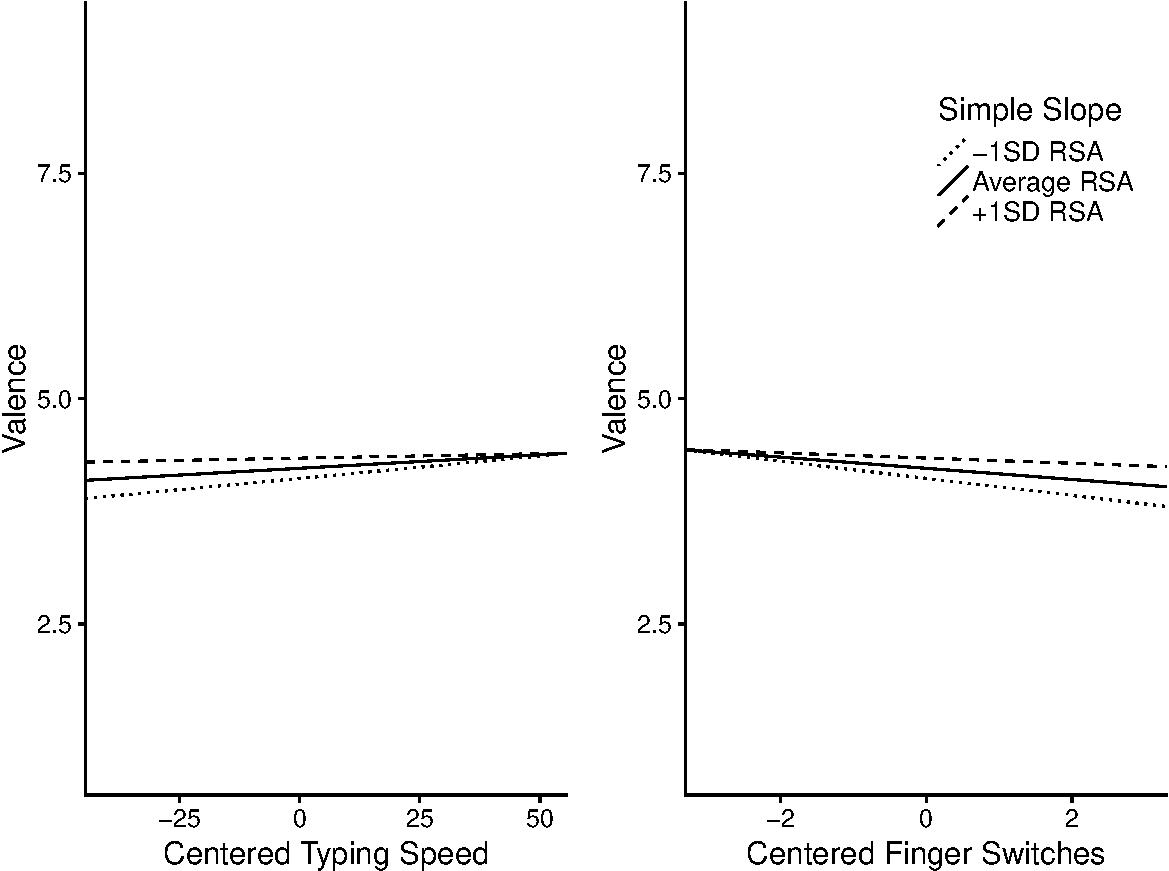
\includegraphics{QWERTY_files/figure-latex/graphs-1.pdf}
\caption{\label{fig:graphs}Simple slopes for pseudowords interaction
effects. The left plot indicates the speed interaction across simple
slopes of RSA, while the right plot indicates the interaction of finger
switches and RSA. Speed has positive effects when RSA is low (left
handed words), while finger switches have negative effects when RSA is
low.}
\end{figure}

\begin{figure}
\centering
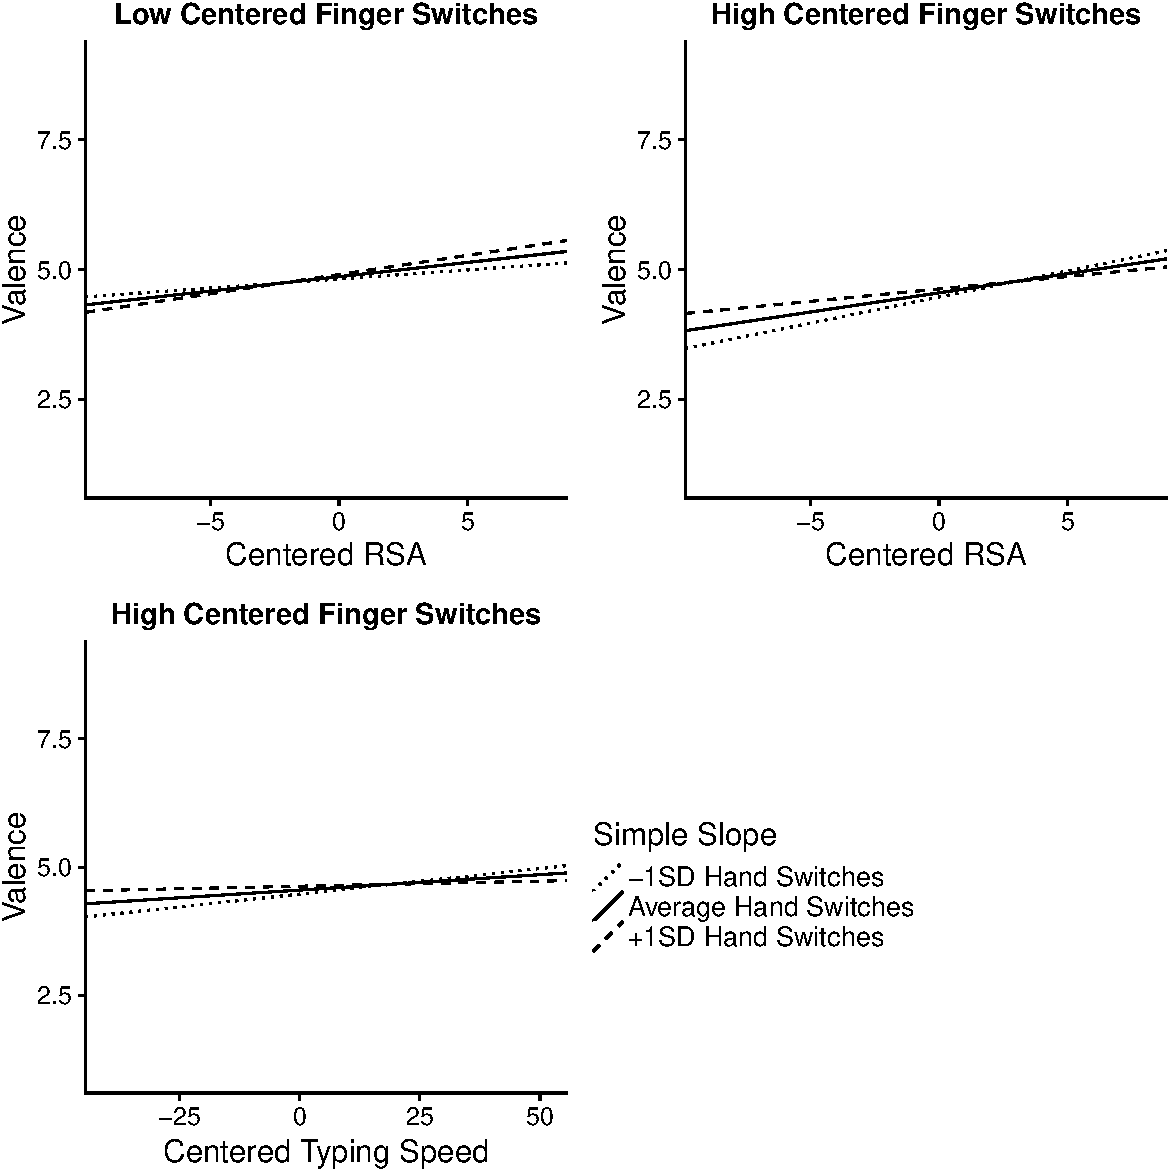
\includegraphics{QWERTY_files/figure-latex/graphs2-1.pdf}
\caption{\label{fig:graphs2}Simple Slopes for real word interactions of
finger switchings by RSA by hand switches and finger switches by speed
by hand switches. The top left figure indicates the interaction for RSA
and hand switches at low finger switches. The average level of finger
switches did not show an interaction. The top right panel portrays the
interaction of RSA and hand switches at high simple slopes for finger
switches. The bottom left figure shows the interaction of typing speed
and hand switches at high finger switches. Low and average finger
switches did not show this interaciton.}
\end{figure}

\section{Discussion}\label{discussion}

These results replicated and extended the QWERTY effect to portray an
interactive view of expertise, typability, and RSA that lead to stronger
valence ratings for words. The QWERTY keyboard layout has influenced our
perceptions of positivity, as hypothesized by the body specificity
hypothesis, but the complexity of typing and action has additionally
lead to changing valence ratings for words. This influence was examined
in our study by incorporating the work of Beilock and Holt (2007),
wherein we measured typing speed as a measure of expertise, as well as
embodied fluency or action through coding the way words would be typed
with finger and hand switches. For pseudowords, we replicated the RSA
effect, and additionally, showed that finger and hand switches predicted
valence ratings. However, both switch variables were negative
predictors, indicating that we dislike words that switch hands and
fingers when adjusting for RSA, speed, and letter frequency. One
interpretation of this finding may be that pseudowords are, by
definition, not traditionally typed, which may have lead participants to
rate words that required hand coordination, along with concentration on
the physical letters, as less positive. If we imagine typing a
\emph{captcha} (i.e., a set of letters and/or numbers designed to
eliminate spam responses), we may find that we would \enquote{peck} at
the keyboard to hit the correct letter combination. Therefore, words
that would require us to use more hands and fingers may be less
desirable.

For real words, the RSA effect was replicated, and both switch variables
predicted valence ratings. In contrast to the pseudowords, we found that
hand switching was a positive predictor of valence, while finger
switching was a negative predictor of valence. Hand switching
coordination would be easier to manage than finger switches, especially
as we consider the flexibility and movement range of the non-index
fingers. Therefore, it appeared that we found words on different hands
as more positive, replicating Beilock and Holt (2007), but when forced
to coordinate switching finger movements, we liked these words less.
Many of the most frequent letters on the QWERTY keyboard are on the left
side, which may frustrate a typist because of the need to coordinate
finger press schemata that involve same finger muscle movements
(Rumelhart \& Norman, 1982). Consequently, the number of switches
becomes increasingly important to help decrease interference from the
need to continue to use the same hand. The ease of action by switching
back and forth is then translated as positive feelings for those fluent
actions (Oppenheimer, 2008). The complexity of this coordination's
effect on valence was found in the multiway interactions unearthed in
this study. Globally, typing speed was not a significant predictor for
pseudo or real words. Viewing expertise through an embodied framework,
it was unclear if speed would directly affect valence, as speed was more
likely to affect our interpretations of typing, rather than positivity.
Therefore, we examined the interaction of typability and speed to
explore how expertise might influence valence through ways that words
are typed.

Pseudowords showed an interaction of typing speed by RSA and finger
switching by RSA when predicting valence. In this interaction, we
focused on RSA as the common variable between these interactions. When
RSA was low, and thus, the words contained more left-handed letters, we
find that speed positively influenced valence, while finger switches
negatively predicted valence. For words typed completely on the right
hand (high RSA), neither variable influence valence. Therefore, it
appears when we are required to use the left hand, and thus, lessened
the influence of RSA, typability and expertise play a role in the
valence ratings of words. Both Beilock and Holt (2007) and van den Bergh
et al. (1990) showed expert preferences for two and three letter
combinations that were typed with different fingers. Our results could
imply that our embodied actions influence preferences for procedures
that are more likely in our environment. While our pseudowords were
legal English phoneme combinations, they are extremely unlikely to have
been previously practiced or encountered in our daily tasks. Therefore,
switching preference will not extend to pseudowords (unpracticed
actions) because they are not fluent (Oppenheimer, 2008).

Further, three-way interactions of finger switches by hand switches by
RSA and finger switches by hand switches by speed were found for real
word valence ratings. Finger switches were first separated in low,
average, and high numbers of switches to see where the two-way
interactions were present. At low finger switches (less than two finger
switches), only the hand switches by RSA interaction was present. This
interaction indicated that increasing hand switches also lead to
increasing effects of RSA on valence. Therefore, when finger switching
competition was low, increased hand switching also lead to increased RSA
effects. This effect indicates that right handed words are still
preferred, but additionally, we find words that are typed with opposite
hands as more positive. At average finger switching, we found no two-way
effects. However, at higher finger switching, we find both a speed and
RSA interaction with hand switching. For RSA, increasing levels of hand
switching lead to lessening the impact of RSA. Therefore, when finger
and hand switching needed to both be coordinated, RSA's impact on
valence decreased but was still significant. For speed, we found that
increasing levels of hand switching also lead to lessened effects of
expertise. This result runs counter to the idea that increased levels of
hand and finger switching would require the most coordination, and thus,
experts should be better at this task. This result instead implies that
the effect of focusing on that coordination may dampen the effects of
expertise on valence ratings.

These embodied results mirror a clever set of studies by Holt and
Beilock (2006) wherein they showed participants sentences that matched
or did not match a set of pictures (i.e., the umbrella is in the air
paired with a picture of an open umbrella). Given dual-coding theory
(Paivio, 1991), it was not surprising that participants were faster to
indicate picture-sentence matches than non-matches (also see Stanfield
\& Zwaan, 2001; Zwaan, Stanfield, \& Yaxley, 2002). Further, they showed
these results extended to an expertise match; hockey and football
players were much faster for sentence-picture combinations that matched
within their sport than non-matches, while novices showed no difference
in speed for matches or non-matches on sports questions. Even more
compelling are results that these effects extend to fans of a sport and
are consistent neurologically (i.e., motor cortex activation in experts;
Beilock, Lyons, Mattarella-Micke, Nusbaum, \& Small, 2008). These
studies clearly reinforce the idea that expertise and fluency
unconsciously affect our choices, even when it comes to perceived
pleasantness of words.

This extension of the QWERTY effect illuminates the need to examine how
skill and action can influence cognitive processes. Additionally, typing
style, while not recorded directly in this experiment, could potentially
illuminate differences in ratings across left-handed and right-handed
words. Hunt-and-peck typists are often slower than the strict typing
manual typists, which may eliminate or change the effects of RSA and
switches since typists may not follow left or right hand rules and just
switch hands back and forth regardless of key position. The middle of a
QWERTY layout also poses interesting problems, as many typists admit to
\enquote{cheating} the middle letters, such as \emph{t}, and \emph{y} or
not even knowing which finger should actually type the \emph{b} key.
Further work could also investigate these effects on other keyboard
layouts, such as Dvorak, which was designed to predominately type by
alternating hands to increase speed and efficiency (Noyes, 1983).

\newpage

\section{References}\label{references}

\setlength{\parindent}{-0.5in} \setlength{\leftskip}{0.5in}

\hypertarget{refs}{}
\hypertarget{ref-Barsalou1999}{}
Barsalou, L. W. (1999). Perceptual symbol systems. \emph{Behavioral and
Brain Sciences}, \emph{22}(4), 577--660.
doi:\href{https://doi.org/10.1017/S0140525X99002149}{10.1017/S0140525X99002149}

\hypertarget{ref-Beilock2007}{}
Beilock, S. L., \& Holt, L. E. (2007). Embodied preference judgments.
\emph{Psychological Science}, \emph{18}(1), 51--57.
doi:\href{https://doi.org/10.1111/j.1467-9280.2007.01848.x}{10.1111/j.1467-9280.2007.01848.x}

\hypertarget{ref-Beilock2008}{}
Beilock, S. L., Lyons, I. M., Mattarella-Micke, A., Nusbaum, H. C., \&
Small, S. L. (2008). Sports experience changes the neural processing of
action language. \emph{Proceedings of the National Academy of Sciences
of the United States of America}, \emph{105}(36), 13269--13273.
doi:\href{https://doi.org/10.1073/pnas.0803424105}{10.1073/pnas.0803424105}

\hypertarget{ref-Bradley1999}{}
Bradley, M. M., \& Lang, P. J. (1999). \emph{Affective Norms for English
Words (ANEW): Instruction manual and affective ratings} (No. C-1). The
Center for Research in Psychophysiology, University of Florida.

\hypertarget{ref-Cartmill2012}{}
Cartmill, E., Goldin-Meadow, S., \& Beilock, S. L. (2012). A word in the
hand: Human gesture links representations to actions.
\emph{Philosophical Transactions of the Royal Society B: Biological
Sciences}, \emph{367}, 129--143.

\hypertarget{ref-Casasanto2009}{}
Casasanto, D. (2009). Embodiment of abstract concepts: Good and bad in
right- and left-handers. \emph{Journal of Experimental Psychology:
General}, \emph{138}(3), 351--367.
doi:\href{https://doi.org/10.1037/a0015854}{10.1037/a0015854}

\hypertarget{ref-Casasanto2011}{}
Casasanto, D. (2011). Different bodies, different minds. \emph{Current
Directions in Psychological Science}, \emph{20}(6), 378--383.
doi:\href{https://doi.org/10.1177/0963721411422058}{10.1177/0963721411422058}

\hypertarget{ref-Davidson1992}{}
Davidson, R. J. (1992). Anterior cerebral asymmetry and the nature of
emotion. \emph{Brain and Cognition}, \emph{20}(1), 125--151.
doi:\href{https://doi.org/10.1016/0278-2626(92)90065-T}{10.1016/0278-2626(92)90065-T}

\hypertarget{ref-Gelman2006}{}
Gelman, A. (2006). Multilevel (hierarchical) modeling: What it can and
cannot do. \emph{Technometrics}, \emph{48}(3), 432--435.
doi:\href{https://doi.org/10.1198/004017005000000661}{10.1198/004017005000000661}

\hypertarget{ref-Glenberg2009}{}
Glenberg, A. M., Webster, B. J., Mouilso, E., Havas, D., \& Lindeman, L.
M. (2009). Gender, emotion, and the embodiment of language
comprehension. \emph{Emotion Review}, \emph{1}(2), 151--161.
doi:\href{https://doi.org/10.1177/1754073908100440}{10.1177/1754073908100440}

\hypertarget{ref-Hauk2004}{}
Hauk, O., Johnsrude, I., \& Pulvermüller, F. (2004). Somatotopic
representation of action words in human motor and premotor cortex.
\emph{Neuron}, \emph{41}(2), 301--307.
doi:\href{https://doi.org/10.1016/S0896-6273(03)00838-9}{10.1016/S0896-6273(03)00838-9}

\hypertarget{ref-Havas2007}{}
Havas, D. A., Glenberg, A. M., \& Rinck, M. (2007). Emotion simulation
during language comprehension. \emph{Psychonomic Bulletin \& Review},
\emph{14}(3), 436--441.
doi:\href{https://doi.org/10.3758/BF03194085}{10.3758/BF03194085}

\hypertarget{ref-Holt2006}{}
Holt, L. E., \& Beilock, S. L. (2006). Expertise and its embodiment:
Examining the impact of sensorimotor skill expertise on the
representation of action-related text. \emph{Psychonomic Bulletin \&
Review}, \emph{13}(4), 694--701.
doi:\href{https://doi.org/10.3758/BF03193983}{10.3758/BF03193983}

\hypertarget{ref-Hommel2001}{}
Hommel, B., Müsseler, J., Aschersleben, G., \& Prinz, W. (2001). The
Theory of Event Coding (TEC): A framework for perception and action
planning. \emph{Behavioral and Brain Sciences}, \emph{24}(05), 849--878.
doi:\href{https://doi.org/10.1017/S0140525X01000103}{10.1017/S0140525X01000103}

\hypertarget{ref-Inhoff1997}{}
Inhoff, A. W., \& Gordon, A. M. (1997). Eye movements and eye-hand
coordination during typing. \emph{Current Directions in Psychological
Science}, \emph{6}(6), 153--157.
doi:\href{https://doi.org/10.1111/1467-8721.ep10772929}{10.1111/1467-8721.ep10772929}

\hypertarget{ref-Jasmin2012}{}
Jasmin, K., \& Casasanto, D. (2012). The QWERTY Effect: How typing
shapes the meanings of words. \emph{Psychonomic Bulletin \& Review},
\emph{19}(3), 499--504.
doi:\href{https://doi.org/10.3758/s13423-012-0229-7}{10.3758/s13423-012-0229-7}

\hypertarget{ref-Lewand2000}{}
Lewand, R. (2000). \emph{Cryptological mathematics}. The Mathematical
Association of America.

\hypertarget{ref-Logan1999}{}
Logan, F. A. (1999). Errors in copy typewriting. \emph{Journal of
Experimental Psychology: Human Perception and Performance},
\emph{25}(6), 1760--1773.
doi:\href{https://doi.org/10.1037//0096-1523.25.6.1760}{10.1037//0096-1523.25.6.1760}

\hypertarget{ref-Logan2003}{}
Logan, G. D. (2003). Simon-type effects: Chronometric evidence for
keypress schemata in typewriting. \emph{Journal of Experimental
Psychology: Human Perception and Performance}, \emph{29}(4), 741--757.
doi:\href{https://doi.org/10.1037/0096-1523.29.4.741}{10.1037/0096-1523.29.4.741}

\hypertarget{ref-Logan1998}{}
Logan, G. D., \& Zbrodoff, N. J. (1998). Stroop-type interference:
Congruity effects in color naming with typewritten responses.
\emph{Journal of Experimental Psychology: Human Perception and
Performance}, \emph{24}(3), 978--992.
doi:\href{https://doi.org/10.1037/0096-1523.24.3.978}{10.1037/0096-1523.24.3.978}

\hypertarget{ref-Lyons2010}{}
Lyons, I. M., Mattarella-Micke, A., Cieslak, M., Nusbaum, H. C., Small,
S. L., \& Beilock, S. L. (2010). The role of personal experience in the
neural processing of action-related language. \emph{Brain and Language},
\emph{112}(3), 214--222.
doi:\href{https://doi.org/10.1016/j.bandl.2009.05.006}{10.1016/j.bandl.2009.05.006}

\hypertarget{ref-Newell1976}{}
Newell, A., \& Simon, H. A. (1976). Computer science as empirical
inquiry: symbols and search. \emph{Communications of the ACM},
\emph{19}(3), 113--126.
doi:\href{https://doi.org/10.1145/360018.360022}{10.1145/360018.360022}

\hypertarget{ref-Noyes1983}{}
Noyes, J. (1983, March). The QWERTY keyboard: a review. Academic Press.
doi:\href{https://doi.org/10.1016/S0020-7373(83)80010-8}{10.1016/S0020-7373(83)80010-8}

\hypertarget{ref-Oppenheimer2008}{}
Oppenheimer, D. M. (2008). The secret life of fluency. \emph{Trends in
Cognitive Sciences}, \emph{12}(6), 237--241.
doi:\href{https://doi.org/10.1016/j.tics.2008.02.014}{10.1016/j.tics.2008.02.014}

\hypertarget{ref-Paivio1991}{}
Paivio, A. (1991). Dual coding theory: Retrospect and current status.
\emph{Canadian Journal of Psychology}, \emph{45}, 255--287.

\hypertarget{ref-Ping2009}{}
Ping, R. M., Dhillon, S., \& Beilock, S. L. (2009). Reach for what you
like: The body's role in shaping preferences. \emph{Emotion Review},
\emph{1}(2), 140--150.
doi:\href{https://doi.org/10.1177/1754073908100439}{10.1177/1754073908100439}

\hypertarget{ref-Pinheiro2017}{}
Pinheiro, J., Bates, D., Debroy, S., Sarkar, D., \& Team, R. C. (2017).
nlme: Linear and nonlinear mixed effects models. Retrieved from
\url{https://cran.r-project.org/package=nlme}

\hypertarget{ref-Rieger2004}{}
Rieger, M. (2004). Automatic keypress activation in skilled typing.
\emph{Journal of Experimental Psychology: Human Perception and
Performance}, \emph{30}(3), 555--565.
doi:\href{https://doi.org/10.1037/0096-1523.30.3.555}{10.1037/0096-1523.30.3.555}

\hypertarget{ref-Rumelhart1982}{}
Rumelhart, D., \& Norman, D. (1982). Simulating a skilled typist: a
study of skilled cognitive-motor performance. \emph{Cognitive Science},
\emph{6}(1), 1--36.
doi:\href{https://doi.org/10.1016/S0364-0213(82)80004-9}{10.1016/S0364-0213(82)80004-9}

\hypertarget{ref-Salthouse1986}{}
Salthouse, T. A. (1986). Perceptual, cognitive, and motoric aspects of
transcription typing. \emph{Psychological Bulletin}, \emph{99}(3),
303--319.
doi:\href{https://doi.org/10.1037/0033-2909.99.3.303}{10.1037/0033-2909.99.3.303}

\hypertarget{ref-Simon1990}{}
Simon, J. R. (1990). The effects of an irrelevant directional cue on
human information processing. In R. Proctor \& T. Reeve (Eds.),
\emph{Stimulus--response compatibility: An integrated perspective} (pp.
31--86). Amsterdam.

\hypertarget{ref-Simon1969}{}
Simon, J. R., \& Small, A. M. (1969). Processing auditory information:
Interference from an irrelevant cue. \emph{Journal of Applied
Psychology}, \emph{53}(5), 433--435.
doi:\href{https://doi.org/10.1037/h0028034}{10.1037/h0028034}

\hypertarget{ref-Stanfield2001}{}
Stanfield, R. A., \& Zwaan, R. A. (2001). The effect of implied
orientation derived from verbal context on picture recognition.
\emph{Psychological Science}, \emph{12}(2), 153--6.
doi:\href{https://doi.org/10.1111/1467-9280.00326}{10.1111/1467-9280.00326}

\hypertarget{ref-Tabachnick2012}{}
Tabachnick, B. G., \& Fidell, L. S. (2012). \emph{Using multivariate
statistics} (6th ed.). Boston, MA: Pearson.

\hypertarget{ref-Tettamanti2005}{}
Tettamanti, M., Buccino, G., Saccuman, M. C., Gallese, V., Danna, M.,
Scifo, P., \ldots{} Perani, D. (2005). Listening to action-related
sentences activates fronto-parietal motor circuits. \emph{Journal of
Cognitive Neuroscience}, \emph{17}(2), 273--281.
doi:\href{https://doi.org/10.1162/0898929053124965}{10.1162/0898929053124965}

\hypertarget{ref-Inc2013}{}
TypingMaster. (2013). TypingTest.com - Complete a Typing Test in 60
Seconds!

\hypertarget{ref-VandenBergh1990}{}
van den Bergh, O., Vrana, S., \& Eelen, P. (1990). Letters from the
heart: Affective categorization of letter combinations in typists and
nontypists. \emph{Journal of Experimental Psychology: Learning, Memory,
and Cognition}, \emph{16}(6), 1153--1161.
doi:\href{https://doi.org/10.1037/0278-7393.16.6.1153}{10.1037/0278-7393.16.6.1153}

\hypertarget{ref-Yang2009}{}
Yang, S.-J., Gallo, D. A., \& Beilock, S. L. (2009). Embodied memory
judgments: A case of motor fluency. \emph{Journal of Experimental
Psychology: Learning, Memory, and Cognition}, \emph{35}(5), 1359--1365.
doi:\href{https://doi.org/10.1037/a0016547}{10.1037/a0016547}

\hypertarget{ref-Zwaan1999}{}
Zwaan, R. A. (1999). Embodied cognition, perceptual symbols, and
situation models. \emph{Discourse Processes}, \emph{28}(1), 81--88.
doi:\href{https://doi.org/10.1080/01638539909545070}{10.1080/01638539909545070}

\hypertarget{ref-Zwaan2006}{}
Zwaan, R. A., \& Taylor, L. J. (2006). Seeing, acting, understanding:
Motor resonance in language comprehension. \emph{Journal of Experimental
Psychology: General}, \emph{135}(1), 1--11.
doi:\href{https://doi.org/10.1037/0096-3445.135.1.1}{10.1037/0096-3445.135.1.1}

\hypertarget{ref-Zwaan2002}{}
Zwaan, R. A., Stanfield, R. A., \& Yaxley, R. H. (2002). Language
comprehenders mentally represent the shapes of objects.
\emph{Psychological Science}, \emph{13}(2), 168--171.
doi:\href{https://doi.org/10.1111/1467-9280.00430}{10.1111/1467-9280.00430}






\end{document}
